%%%%%%%%%%%%%%%%%%%%%%%%%%%%%%%%%%%%%%%%%%%%%%%%%%%%%%%%%%%%%%%%%%%%%%%%%%%%%%%%
%2345678901234567890123456789012345678901234567890123456789012345678901234567890
%        1         2         3         4         5         6         7         8

\documentclass[letterpaper, 10 pt, conference]{ieeeconf}  % Comment this line out if you need a4paper

%\documentclass[a4paper, 10pt, conference]{ieeeconf}      % Use this line for a4 paper

\IEEEoverridecommandlockouts                              % This command is only needed if 
                                                          % you want to use the \thanks command

\overrideIEEEmargins                                      % Needed to meet printer requirements.

% See the \addtolength command later in the file to balance the column lengths
% on the last page of the document

% The following packages can be found on http:\\www.ctan.org
%\usepackage{graphics} % for pdf, bitmapped graphics files
%\usepackage{epsfig} % for postscript graphics files
%\usepackage{mathptmx} % assumes new font selection scheme installed
%\usepackage{times} % assumes new font selection scheme installed
%\usepackage{amsmath} % assumes amsmath package installed
%\usepackage{amssymb}  % assumes amsmath package installed
\usepackage{graphicx}
\usepackage[export]{adjustbox}
\graphicspath{ {images/} }


\title{\LARGE \bf
DuckieGuard
}


\author{Chang-Yan Li$^{1}$, Chong-Sin Huang$^{2}$, Hao-Yun Chen$^{2}$, Shih-Jie Chang$^{2}$, Yi-Lun Wu$^{2}$% <-this % stops a space
\thanks{*This work was supported by the Robotics Master Program in National Chiao Tung University, Taiwan}% <-this % stops a space
\thanks{$^{1}$Chang-Yan Li is with National Chiao Tung University, Taiwan.
        {\tt\small avneger2236@gmail.com}}%
\thanks{$^{2}$Chong-Sin Huang, Hao-Yun Chen, Shih-Jie Chang, Yi-Lun Wu
        {\tt\small b.d.researcher@ieee.org}}%
}


\begin{document}
\maketitle
\pagestyle{empty}

\section{INTRODUCTION \& MOTIVATION}
With people’s rising awareness of their own safety, various monitoring machine have been applied to our surroundings. People expect these machine to prevent potential crimes from happening and thus guarantee their safety. Indeed, it works, but it’s not enough. Lack of the ability to move makes these machine predictable, while lack of the ability to detect danger makes it only useful after events take place. To solve these problems, we decide to develop this application – DuckieGuard, which is able to move, detect dangers and send warning messages to owners. 

As for moving ability, our DuckieGuard will patrol between two checking points that would have been set previously by users. When meeting the checking points, DuckieGuard will stop and check whether there is anything suspicious. In this way, we can make our DuckieGuard less predictable and more flexible with changeable checking points set by users.

When it comes to danger detection, we plan to enable our DuckieGuard to recognize dangerous things using deep learning. It is when located at checking points that DuckieGuard will implement this function. When detecting something suspicious, DuckieGuard will send warning messages to the user’s cellphone. In this way, users can get instant information of coming danger and thus able to avoid it.

To sum up, DuckieGuard will be especially distinctive when it comes to its flexibility and instantaneity. Users can set checking points by themselves and receive instant warning messages. In this way, we hope this application can provide users with more protection and a profounder sense of safety.

\section{SYSTEM ARCHITECTURE \& EQUIPMENTS}
\label{section:system_architecture}
\subsection{SYSTEM ARCHITECTURE}
The system block diagram is showned in Fig.~\ref{figure:system_block_diagram}.
Guard\_node is the core controller in this system. 
It subscribes to object\_recognition\_node for recognition results.
When any unusual object is detected, the guard\_node publishs messages
to lane\_controller\_node and notification\_node which control
duckiebot and deliver notifications respectively; then all notifications are sent to
our http server. User agent can request for notifications from the server.
After user receives notifications,
he can control the duckiebot to do some helpful things via mobile device.

Core techniques of each node:
\begin{itemize}
  \item Guard\_node: Flow control.
  \item Object\_recognition\_node: OpenCV or TensorFlow.
  \item Lane\_controller\_node: Lane following.
  \item Inverse\_kinematics\_node: Use buildin node.
  \item Notification\_node: HTTP request or WebSocket, thread handling.
\end{itemize}

Server side techniques:
\begin{itemize}
  \item Django
  \item HTTP request, WebSocket
\end{itemize}

User agent techniques:
\begin{itemize}
  \item Android
  \item HTTP request, WebSocket
\end{itemize}

\subsection{EQUIPMENTS} 
The system doesn't need extra hardware on duckiebot(Fig.~\ref{figure:duckiebot}),
but need a computer to run the server, and a mobile device to receive notification.

\begin{figure}[t] % h means put this image here
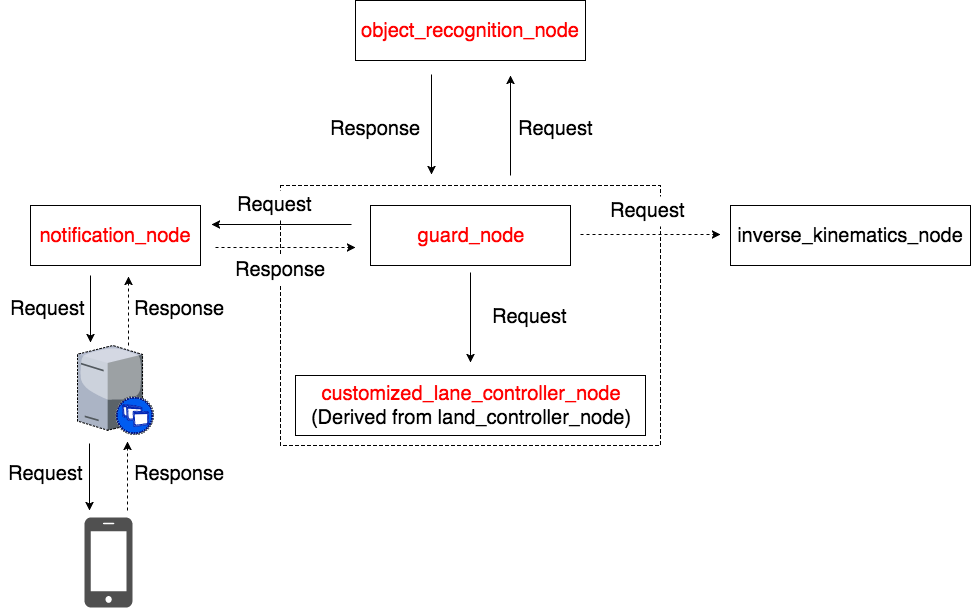
\includegraphics[width=1\columnwidth]{csp2017}
\centering
\caption{System block diagram. Red text are the nodes which should be implemented. Dashed lines ara the optional architecture.}
\label{figure:system_block_diagram}
\end{figure}

\begin{figure}[t] % h means put this image here
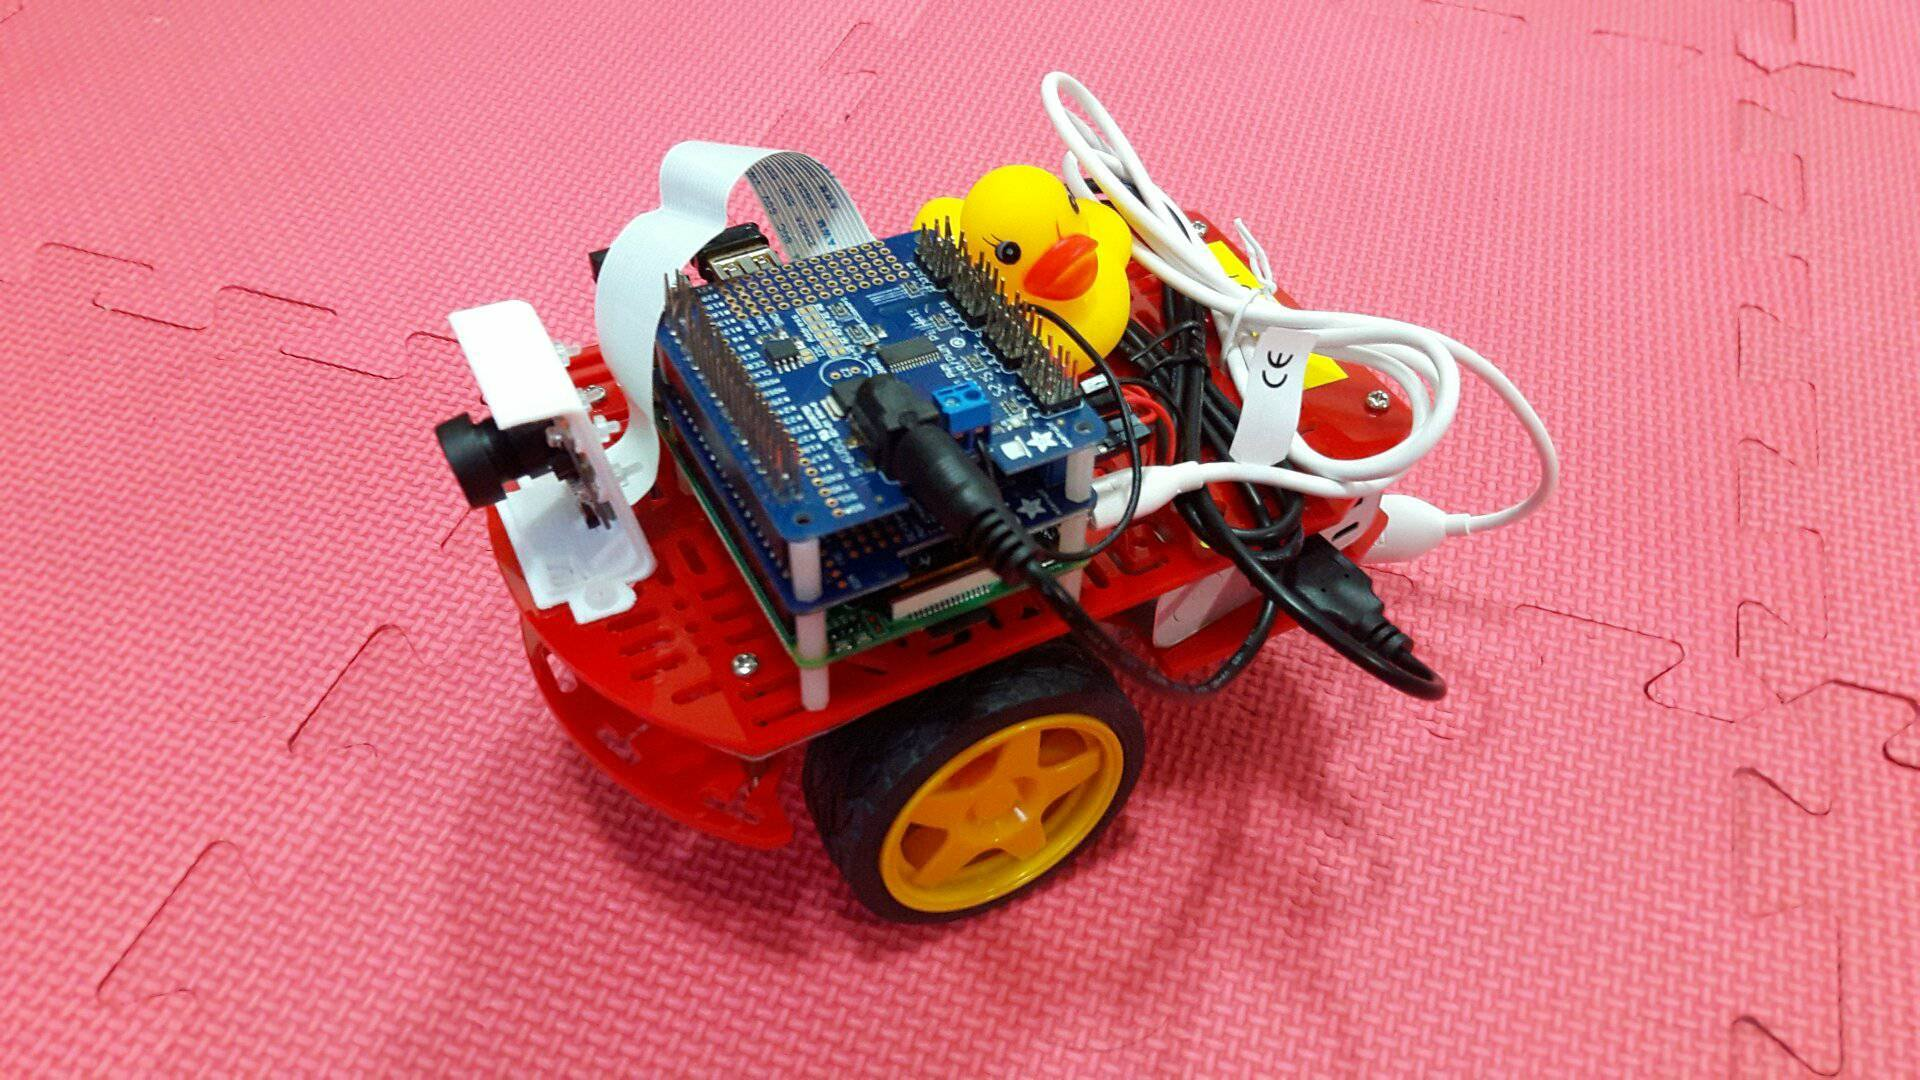
\includegraphics[width=0.8\columnwidth]{duckiebot}
\centering
\caption{Duckiebot.}
 \label{figure:duckiebot}
\end{figure}

\section{SPECIFIC AIMS}

I am responsible for the design of the Guard\_node. Including Flow control(Using Finite-state machine) and the center control api -- consolidate all of the data from other node.

\begin{itemize}
\item Flow control -- Finite-state machine
\item Center control api
\end{itemize}

\section{APPROACH}

In order to finish my work,I will use the Finite-state machine theory. The guard\_node will keep request and get the response of object\_recongnition\_node. If the duckieguard find the intruder, request to notification\_node in order to let the user know. Besides, if user wants to control the duckieguard by himself/herself, guard\_node will response what duckieguard see and accept the request of user. Last but not least, request Lane\_controller\_node by the result of all of the imformations.
In order to do my work better, I will need to know preliminary knowledge of other nodes.

\section{SCHEDULE AND TEAM COLLABORATION}

In the first two week, I will finish the first version of the Finite-state machine, and then start to design the center control api. That means other members nead to finish the first version of the node. In my opinion, it will be better to finish the first version of center control api in one month, so that we have sufficient time to debug. After the attemption for the first month, I will finish a complete (but not perfect enough ) version of the center control api. In the last period before the dead line, I will keep revise the center control api to make it perfect. Besides, if there are some new function of duckieguard, I will finish it during the period of the time. 
   

\addtolength{\textheight}{-12cm}   % This command serves to balance the column lengths
                                  % on the last page of the document manually. It shortens
                                  % the textheight of the last page by a suitable amount.
                                  % This command does not take effect until the next page
                                  % so it should come on the page before the last. Make
                                  % sure that you do not shorten the textheight too much.

\bibliographystyle{IEEEtran}
\bibliography{egbib}

\end{document}
